
\chapter{Programming Model}

The programming model Kokkos is characterized by 6 core abstractions: Execution Spaces, Execution Patterns, Execution Policies, Memory Spaces, Memory Layout and Memory Traits. 
These abstraction concepts allow the formulation of generic algorithms and data structures which can then be mapped to different types of architectures. 
Effectively they allow for compile time transformation of algorithms to allow for adaptions of varying degrees of hardware parallelism as well as of the memory hierarchy. 

\begin{figure}[h]
\begin{center}
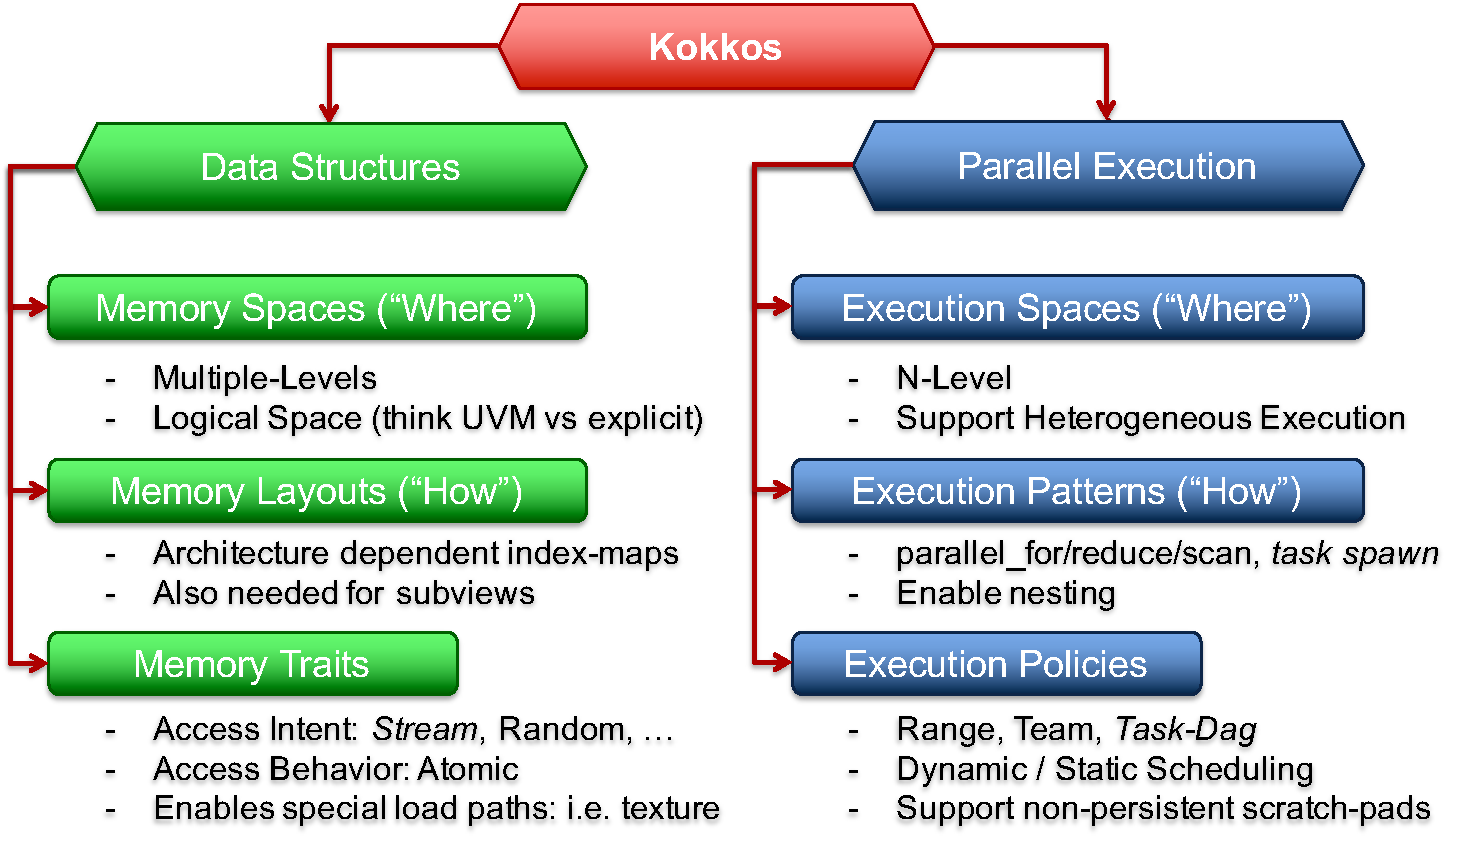
\includegraphics[clip, trim=1cm 5.5cm 12cm 2.5cm, width=\textwidth]{figures/kokkos-abstractions.pdf}
\caption{The core abstractions of the Kokkos Programming Model}
\label{fig:kokkosabstractions}
\end{center}
\end{figure}

\section{Execution Spaces}

An Execution Space is the place {\it Where} code can actually be executed. 
For example on current Hybrid GPU / CPU systems there are two types of execution spaces: the GPU cores and the CPU cores. 
In the future this could include Processing in Memory (PIM) modules or different core types on a heterogenous CPU.
In principle this can also be used to introduce remote memory spaces, e.g. the capability of sending work to a different node.
Execution Spaces thus give an application developer the means to target different parts of a heterogenous hardware architecture.
This corresponds directly to the previously described machine model.

\section{Execution Patterns}

Execution Patterns are the fundamental parallel algorithms in which an application has to be expressed.
Examples are \lstinline|parallel_for|: execute a function in undeterminded order a specified amount of times.,
\lstinline|parallel_reduce|: which combines a \lstinline|parallel_for| execution with a reduction operation,
\lstinline|parallel_scan|: which combines a \lstinline|parallel_for| operation with a prefix or postfix scan on output values of each operation, and
\lstinline|task|: which executes a single function with dependencies on other functions.
Expressing an application in these patterns allows the underlying implementation or the used compiler to reason about valid transformations.
For example all \lstinline|parallel_***| patterns allow unspecified execution order, and only promise deterministic results of the reductions themselves.
This enables different mapping patterns on different hardware such as assignment of iterations to threads or vector lanes. 

\section{Execution Policies}

An Execution Policy determines together with an Execution Pattern {\it How} a function is executed.
Some policies can be nested in others.

\subsection{Range Policies}

The most simple form of execution policies are {\it Range Policies}. 
They are used to execute an operation once for each element in a range. 
There are no prescriptions of order of execution or concurrency, which means that it is not legal
to synchronize different iterations. 

\subsection{Team Policies}

Team policies are used to implement hierarchical parallelism. 
For that purpose Kokkos groups threads into \emph{teams}.
A \emph{thread team} is a collection of one or more parallel ``threads'' of execution.
Kokkos allows an arbitrary number of teams -- the \emph{league size}.
Hardware constrains the number of threads in a team -- the \emph{team size}.
All threads in a team are guaranteed to run concurrently. 

Threads in a team can synchronize -- they have a ``barrier'' primitive -- 
and share a ``scratch pad'' memory which they may use for temporary storage.
Note that not all forms of synchronization mechanism are legal in Kokkos, in particular
implementing ``spin-locks'' for threads in a team may result in dead locks. 
In Kokkos there is no forward progress guarantee for threads, that means that a single thread spinning
on a lock acquired by another thread of the team may use 100\% of the compute engines resources.
Calling the explicit Kokkos team barrier is the only safe way to synchronize threads in a team.

Scratch pad memory exists only during parallel operations;
allocations in it do not persist across kernels.
Teams themselves may run in any order,
and may not necessarily run all in parallel.
For example, if the user asks for $T$ teams,
the hardware may choose to run them one after another in sequence,
or in groups of up to $G$ teams at a time in parallel.

Users may \emph{nest} parallel operations.
Teams may perform one parallel operation (for, reduce, or scan),
and threads within each team may perform another, possibly different parallel operation.
Different teams may do entirely different things.
For example, all the threads in one team may execute a \lstinline!parallel_for!,
and all the threads in a different team may execute a \lstinline!parallel_scan!.
Different threads within a team may also do different things.
However, performance may vary if threads in a team ``diverge'' in their behavior
(e.g., take different sides of a branch).
Chapter \ref{C:Hierarchical} shows how the C++ implementation of Kokkos exposes thread teams.

NVIDIA's CUDA programming model inspired Kokkos' thread team model.
The scratch pad memory corresponds with CUDA's per-team ``shared memory.''
The ``league / team'' vocabulary comes from OpenMP 4.0,
and has many aspects in common with our thread team model.
We have found that programming to this model results in good performance,
even on computer architectures which only implement parts of the full model.
For example, most multicore processors in common use for high-performance computing lack ``scratch pad'' hardware.
However, if users request a scratch pad size that fits comfortably in the largest cache shared by the threads in a team,
programming as if a scratch pad exists forces users to address locality in their algorithms.
This also reflects the common experience that rewriting a code for more restrictive hardware,
then porting the code \emph{back} to conventional hardware,
tends to improve performance relative to an unoptimized code.

\section{Memory Spaces}

Memory Spaces are the places {\it Where} data resides.
They specify physical location of data as well as certain access characteristics. 
Different physical locations correspond to things such as high bandwidth memory, on die scratch memory or non-volatile bulk storage.
Different logical memory spaces allow for concepts such as UVM memory in the CUDA programming model, which is accessible from Host and GPU. 
Memory Spaces also could in the futrue also be used to express remote memory locations.
Furthermore they encapsulate functionality such as consistency control and persistence scopes.

\section{Memory Layout}

Layouts express the mapping from logical (or algorithmical) indicies to address offset for a data allocation. 
By adopting appropriate layouts for memory structures an application can optimise data access patterns in a given algorithm.
If an implementation provides polymorphic layouts (i.e. a data structure can be instantiated at compile or runtime with different layouts) an architecture dependent optimisation can be performed.

\section{Memory Traits}

Memory Traits specify how a data structure is accessed in an algorithm. 
Traits express usage scenarios such as atomic access, random access and streaming loads or stores.
By putting such attributes on data structures, an implementation of the programming model can insert optimal load and store operations.
If a compiler implements the programming model, it could reason about the access modes and use that to inform code transformations.   

